\documentclass{article}

\usepackage{booktabs}
\usepackage{tabularx}
\usepackage{graphicx}

\title{SE 3XA3: Problem Statement\\Spann}

\author{Team 8
		\\ Christopher Stokes | stokescd
		\\ Varun Hooda | hoodav
}

\date{}

%% Comments

\usepackage{color}

\newif\ifcomments\commentstrue

\ifcomments
\newcommand{\authornote}[3]{\textcolor{#1}{[#3 ---#2]}}
\newcommand{\todo}[1]{\textcolor{red}{[TODO: #1]}}
\else
\newcommand{\authornote}[3]{}
\newcommand{\todo}[1]{}
\fi

\newcommand{\wss}[1]{\authornote{blue}{SS}{#1}}
\newcommand{\ds}[1]{\authornote{red}{DS}{#1}}
\newcommand{\mj}[1]{\authornote{red}{MSN}{#1}}
\newcommand{\cm}[1]{\authornote{red}{CM}{#1}}
\newcommand{\mh}[1]{\authornote{red}{MH}{#1}}

% team members should be added for each team, like the following
% all comments left by the TAs or the instructor should be addressed
% by a corresponding comment from the Team

\newcommand{\tm}[1]{\authornote{magenta}{Team}{#1}}


\begin{document}

\begin{table}[hp]
\caption{Revision History} \label{TblRevisionHistory}
\begin{tabularx}{\textwidth}{llX}
\toprule
\textbf{Date} & \textbf{Developer(s)} & \textbf{Change}\\
\midrule
    Sept. 26, 2016 & Christopher, Varun & Initial development plan\\
    Sept. 28, 2016 & Varun & Formatting, Introduction and Git Workflow\\
    Sept. 29, 2016 & Christopher, Varun & Changes to wording and added Proof of
    Concept plan section\\
\bottomrule
\end{tabularx}
\end{table}

\newpage

\maketitle

This document outlines some key points regarding the development of this
project. The points discussed related to the way the team will work (meetings,
workflow, communication) and how the project will undergo development and
progress as time goes on.

\section{Team Meeting Plan}
The team will meet on a weekly basis on Tuesday afternoons on campus (exact
location and time is up to the discretion of the team members). The meetings
will allow the team to express any concerns, discuss upcoming
deadlines/milestones, and discuss the work plan for the upcoming week. Team
members will alternate as the chair for each meeting. The chair will be
responsible for creating an appropriate agenda for the weeks meeting and for
directing the meeting.

\section{Team Communication Plan}
The primary means of communication will be Google Hangouts. Issue tracking on
gitlab will be used for formally discussing any issues with the project.

\section{Team Member Roles}
There will be no team leader due the small team size. A team member may lead
the team for a particular task if the team member is experienced in that
particular task.
Roles will be as follows:
\begin{description}
  \item[Christopher Stokes] Primarily work on backend server code, as well as
    some work on the custom framework that will be used and on some frontend
    code. Will be the expert on the technologies used on this project.
  \item[Varun Hooda] Primarily work on frontend code, as well as on the custom
    framework. Will be the expert on \LaTeX
\end{description}

\section{Git Workflow Plan}
Git and Gitlab will be used to manage the project's documentation and code
base. The team will use a single repository (no forks) with all developers
contributing to the same code base. Git branches will be used to reduce
conflicts between different incomplete features The team will attempt to commit
and push changes frequently. Labels will be used to differentiate or highlight
particular milestones.

\section{Proof of Concept Demonstration Plan}
The goal of the demonstration plan is to identify any risks that the team may
not be able to overcome. In preparation for the demonstration, the team will
build a prototype of the final project that will be used to highlight the
primary goal of the project. This prototype may highlight the issues previously
mentioned, thus help the team move forward by either redefining the project
scope or adjusting the project to avoid the risk. The prototype itself will be
a simplified version of the final software, including only the key critical
features that are vital to the project or features that have a significant risk
attached to them.

The goal of the demonstration, essentially, is to highlight any of the
following possible issues:
\begin{itemize}
  \item Implementation problems
    \begin{itemize}
      \item Feature implementation is beyond the skill level of the team
        members
      \item Feature is infeasible to implement
      \item Feature implementation would require too much time
      \item Feature implementation would require resources beyond the groups
        means
    \end{itemize}
  \item Verify the project can be tested and verified
    \begin{itemize}
      \item Will there be some feature or part of the project that is
        impossible/infeasible/impractical to test and ensure correctness of
    \end{itemize}
  \item All software/hardware dependencies are satisfiable
    \begin{itemize}
      \item Will the team be able to setup the required supporting hardware and
        software to allow the project to run
    \end{itemize}
  \item Issues running the prototype on different devices
    \begin{itemize}
      \item Will the project be able to provide the same functionality on
        different platforms, operation systems, and browsers
    \end{itemize}
  \item The final project will be able to do what is specified
    \begin{itemize}
      \item The project goals can be implemented and the final project will be
        able to meet the specification requirements
    \end{itemize}
\end{itemize}

% During the demonstration itself, the majority of problems could arise from
% issues connecting to the server or database due to firewall or network
% preferences. To ensure that this does not occur during the demo, the server and
% database will be hosted locally on the computer running the web app. This
% minimises all connection issues as the connection is local so the firewall and
% outside network will have no effect on the connection.

\section{Technology}
The project will use modern web technologies for the frontend: HTML5, CSS3
(compiled from LESS) and JavaScript. The backend server will run C\# code and
use the PostgreSQL object-relational database management system (ORDBMS) to
store and retrieve data. A custom JavaScript web framework will also be used to
create the frontend website (to avoid manually writing HTML).

For testing, the project will use Postman for the API, Jasmine for JavaScript
and Nunitfor C\#.

For documentation generation, the project will use C\# source code
documentation and Doxygen.

\section{Coding Style}
The project will the following coding styles for all of the code:
\begin{itemize}
  \item ECMA5 Script Standard for JavaScript
  \item LESS Standard for LESS files
  \item Microsoft Coding Conventions for C\#
\end{itemize}

\section{Project Schedule}

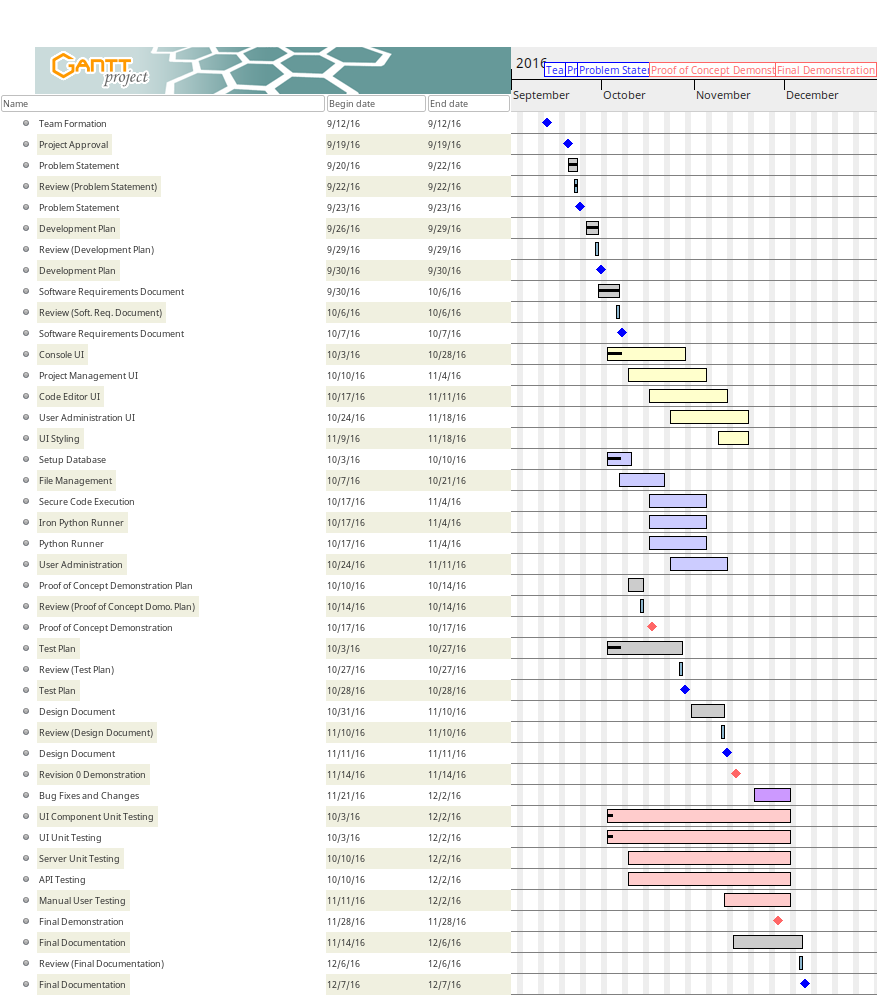
\includegraphics[width=\textwidth]{../ProjectSchedule/schedule}

\section{Project Review}

\end{document}
